% !TEX root = ../main.tex
\chapter{Modello del dominio e cicli di vita}
\label{cap:dominio}
\section{Concetti e relazioni del dominio}
In questo capitolo è presentato il modello del dominio, con le entità principali e le loro relazioni. Il modello è stato suddiviso in 3 sottodiagrammi per motivi di leggibilità, ma tutti i diagrammi rappresentano parti collegate dello stesso modello.

\subsection{Utenti, ruoli e moderazione}
\label{sec:dominio-utenti}
\texttt{User} rappresenta un account registrato, contiene i propri dati anagrafici, contatti, lo stato dell'account (\texttt{AccountStatus}, che può essere \texttt{ACTIVE} oppure \texttt{BANNED}) e il flag \texttt{isAdmin}. La password è gestita separatamente e non è visibile nel modello del dominio. Administrator e Organiser non sono classi distinte, ma ruoli assegnati a un \texttt{User}, tramite il flag \texttt{isAdmin} per l'amministratore e all'interno di un \texttt{Event} specifico per l'organizzatore (vedi sezione~\ref{sec:dominio-eventi}).

La moderazione degli account è gestita dagli amministratori, che possono compilare dei \texttt{Report}, ciascun report collega un amministratore a uno \texttt{User} segnalato e facoltivamente a un \texttt{Event}. Il report è composto dalla severità (\texttt{ReportSeverity}), dalla data di creazione e da un commento. La severità può essere \texttt{LOW}, \texttt{MIDDLE} o \texttt{HIGH}. I ban e i report sono operazioni distinte, senza automatismi, i report possono essere consultati dagli amministratori, che possono poi decidere se cambiare lo stato dell'account segnalato in \texttt{BANNED} oppure lasciarlo \texttt{ACTIVE}.
\begin{figure}[!htbp]
  \centering
  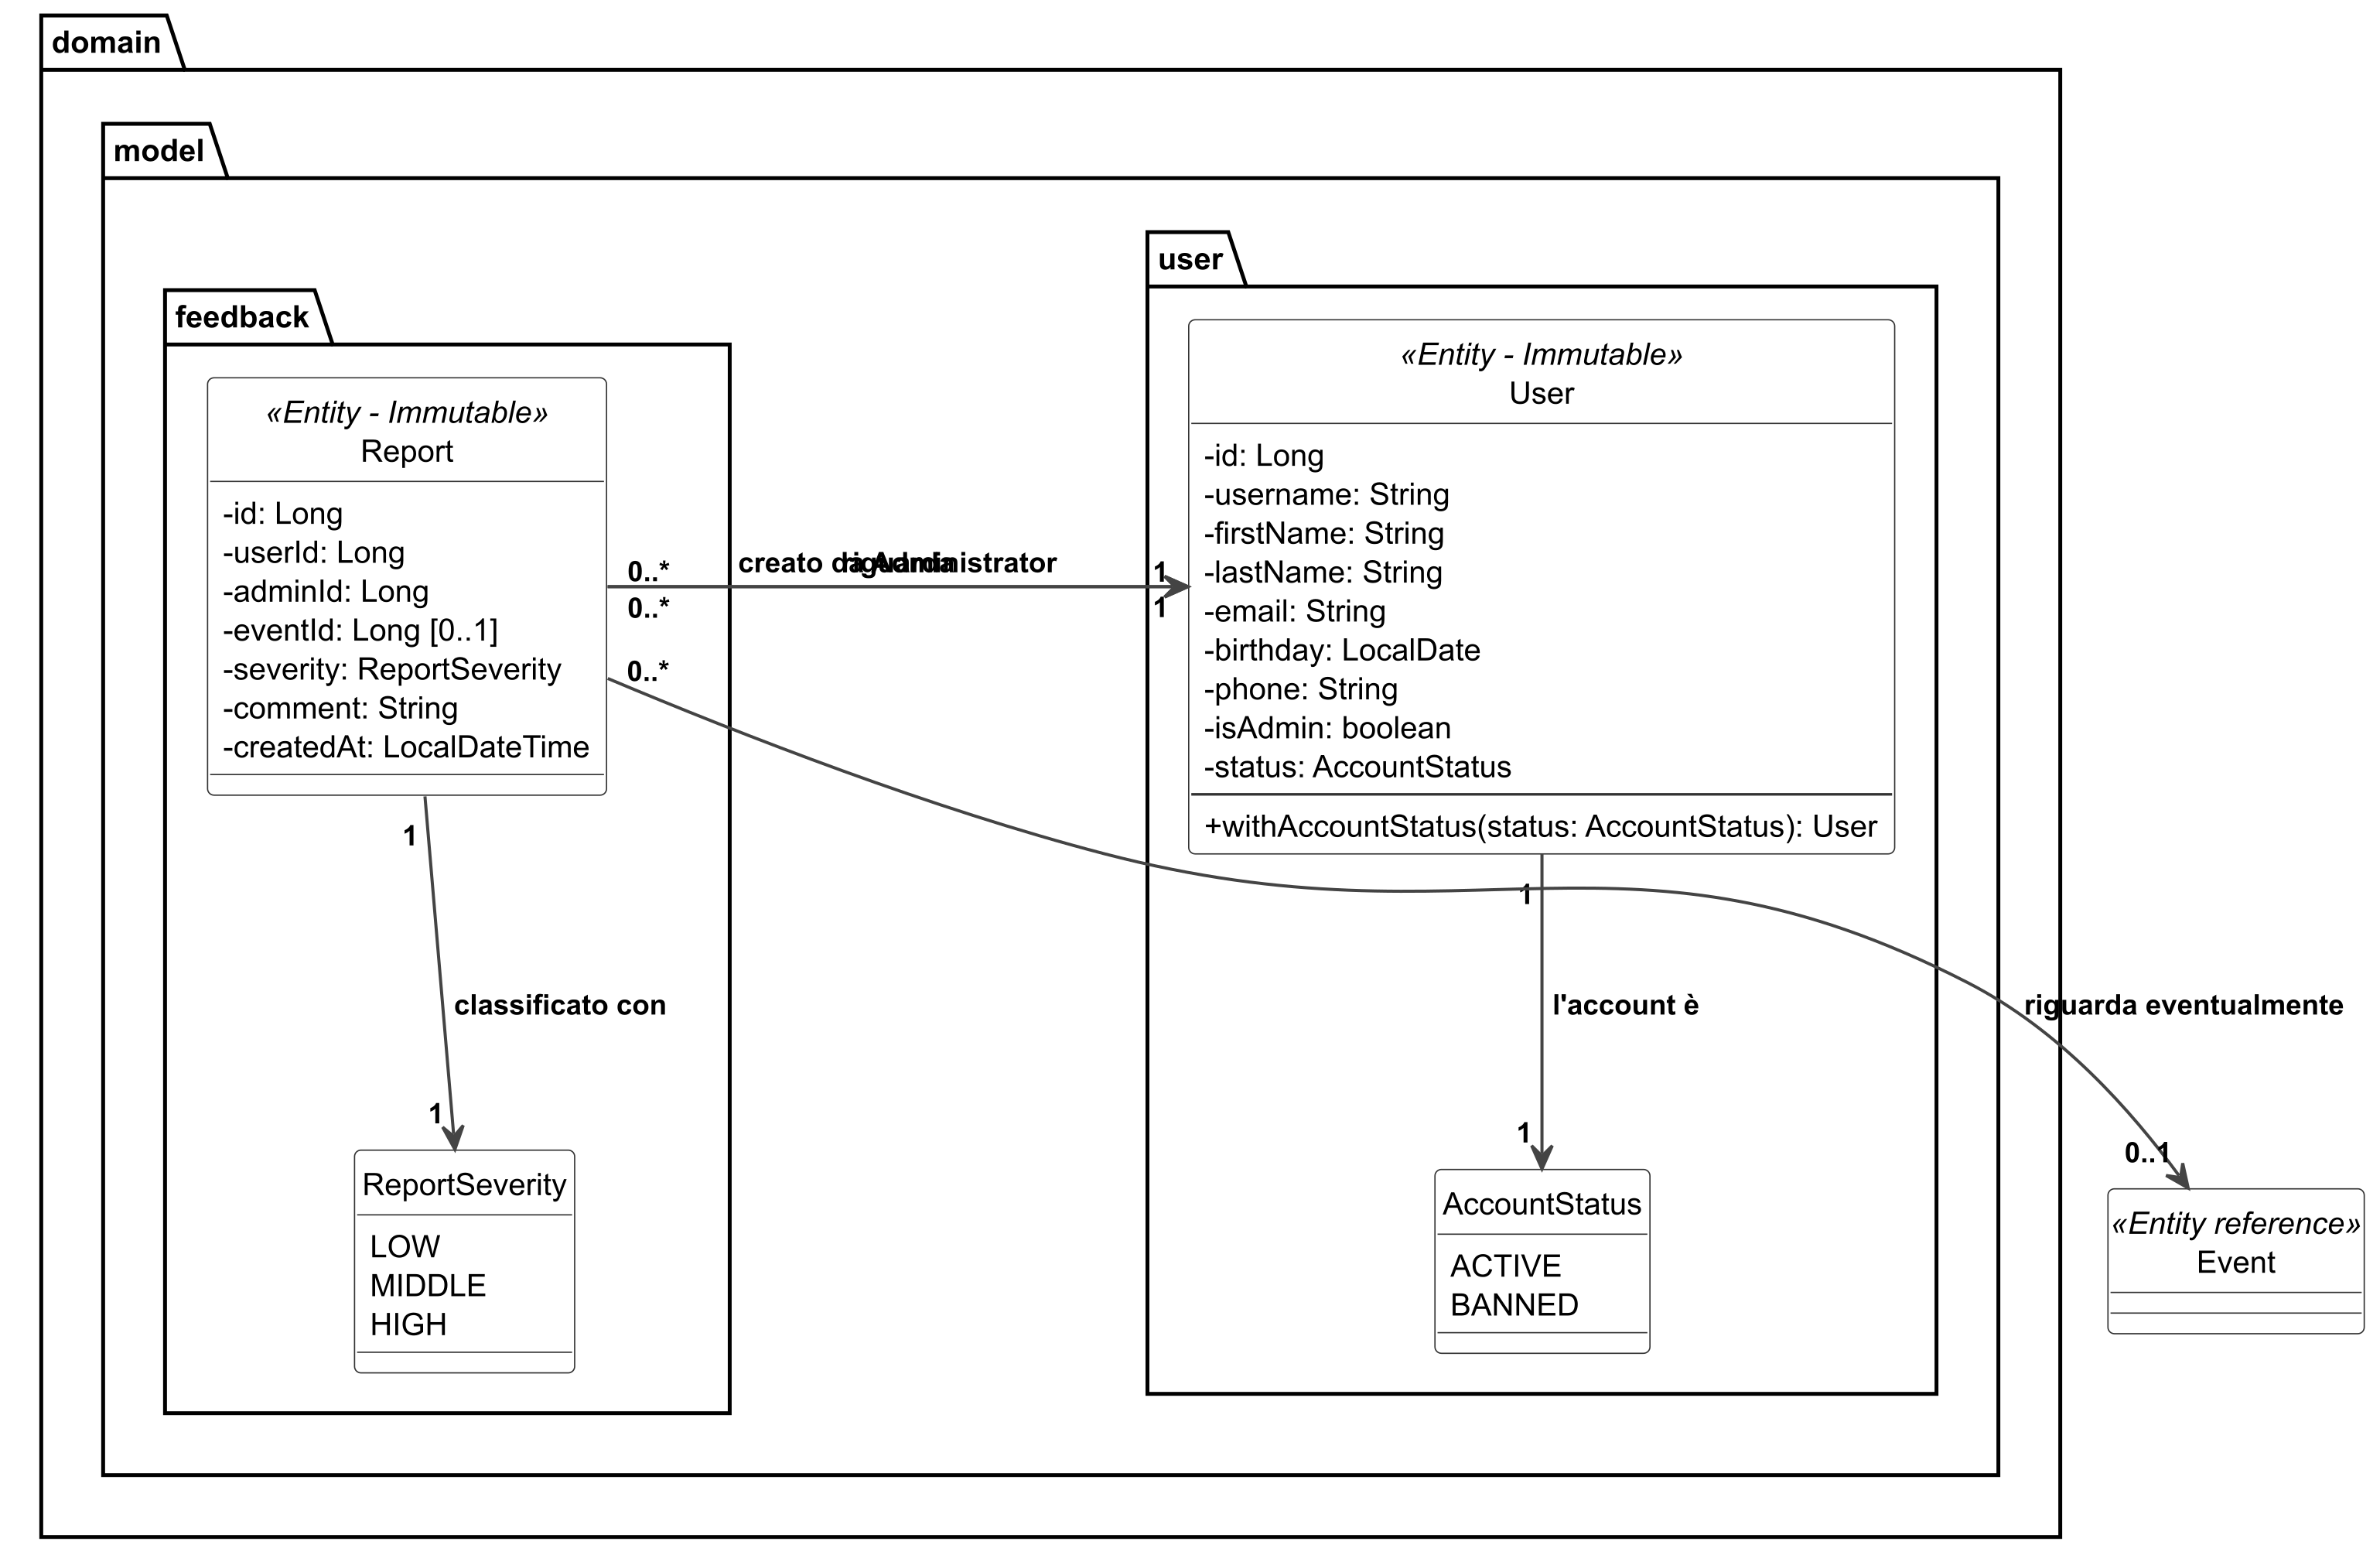
\includegraphics[width=\textwidth,height=0.28\textheight,keepaspectratio]{dominio/domain-users.png}
  \caption{Diagramma del dominio: utenti e moderazione.}
  \label{fig:dominio-utenti}
\end{figure}
\FloatBarrier
\par\medskip

\clearpage
\subsection{Venue e risorse}
\label{sec:dominio-risorse}
Una \texttt{Venue} rappresenta un luogo fisico in cui è possibile organizzare eventi. Possiede un nome, una descrizione e un indirizzo (\texttt{Address} che raggruppa i dati dell'indirizzo).
Una \texttt{Resource} è invece un qualche tipo di risorsa, collegata a una venue o meno, che può opzionalmente essere associata a una richiesta o a un evento.
\texttt{Resource} è una classe astratta, da cui derivano tre sottoclassi concrete:
\begin{itemize}
  \item \texttt{Space}, che rappresenta uno spazio fisico, come una sala o un palco, appartenente a una venue;
  \item \texttt{Equipment}, che rappresenta un'attrezzatura, come un proiettore o un microfono. Può appartenere a una venue oppure essere globale, cioè non legata a una venue specifica. Per le attrezzature è possibile definire una quantità totale disponibile;
  \item \texttt{Service}, che rappresenta un servizio, come il catering o la sicurezza. I servizi sono globali, ovvero non legati a una venue particolare.
\end{itemize}
Una venue può disporre di zero o più spazi e attrezzature. Ogni spazio appartiene a una sola venue, mentre un'attrezzatura può essere associata a zero o una venue.
\begin{figure}[!htbp]
  \centering
  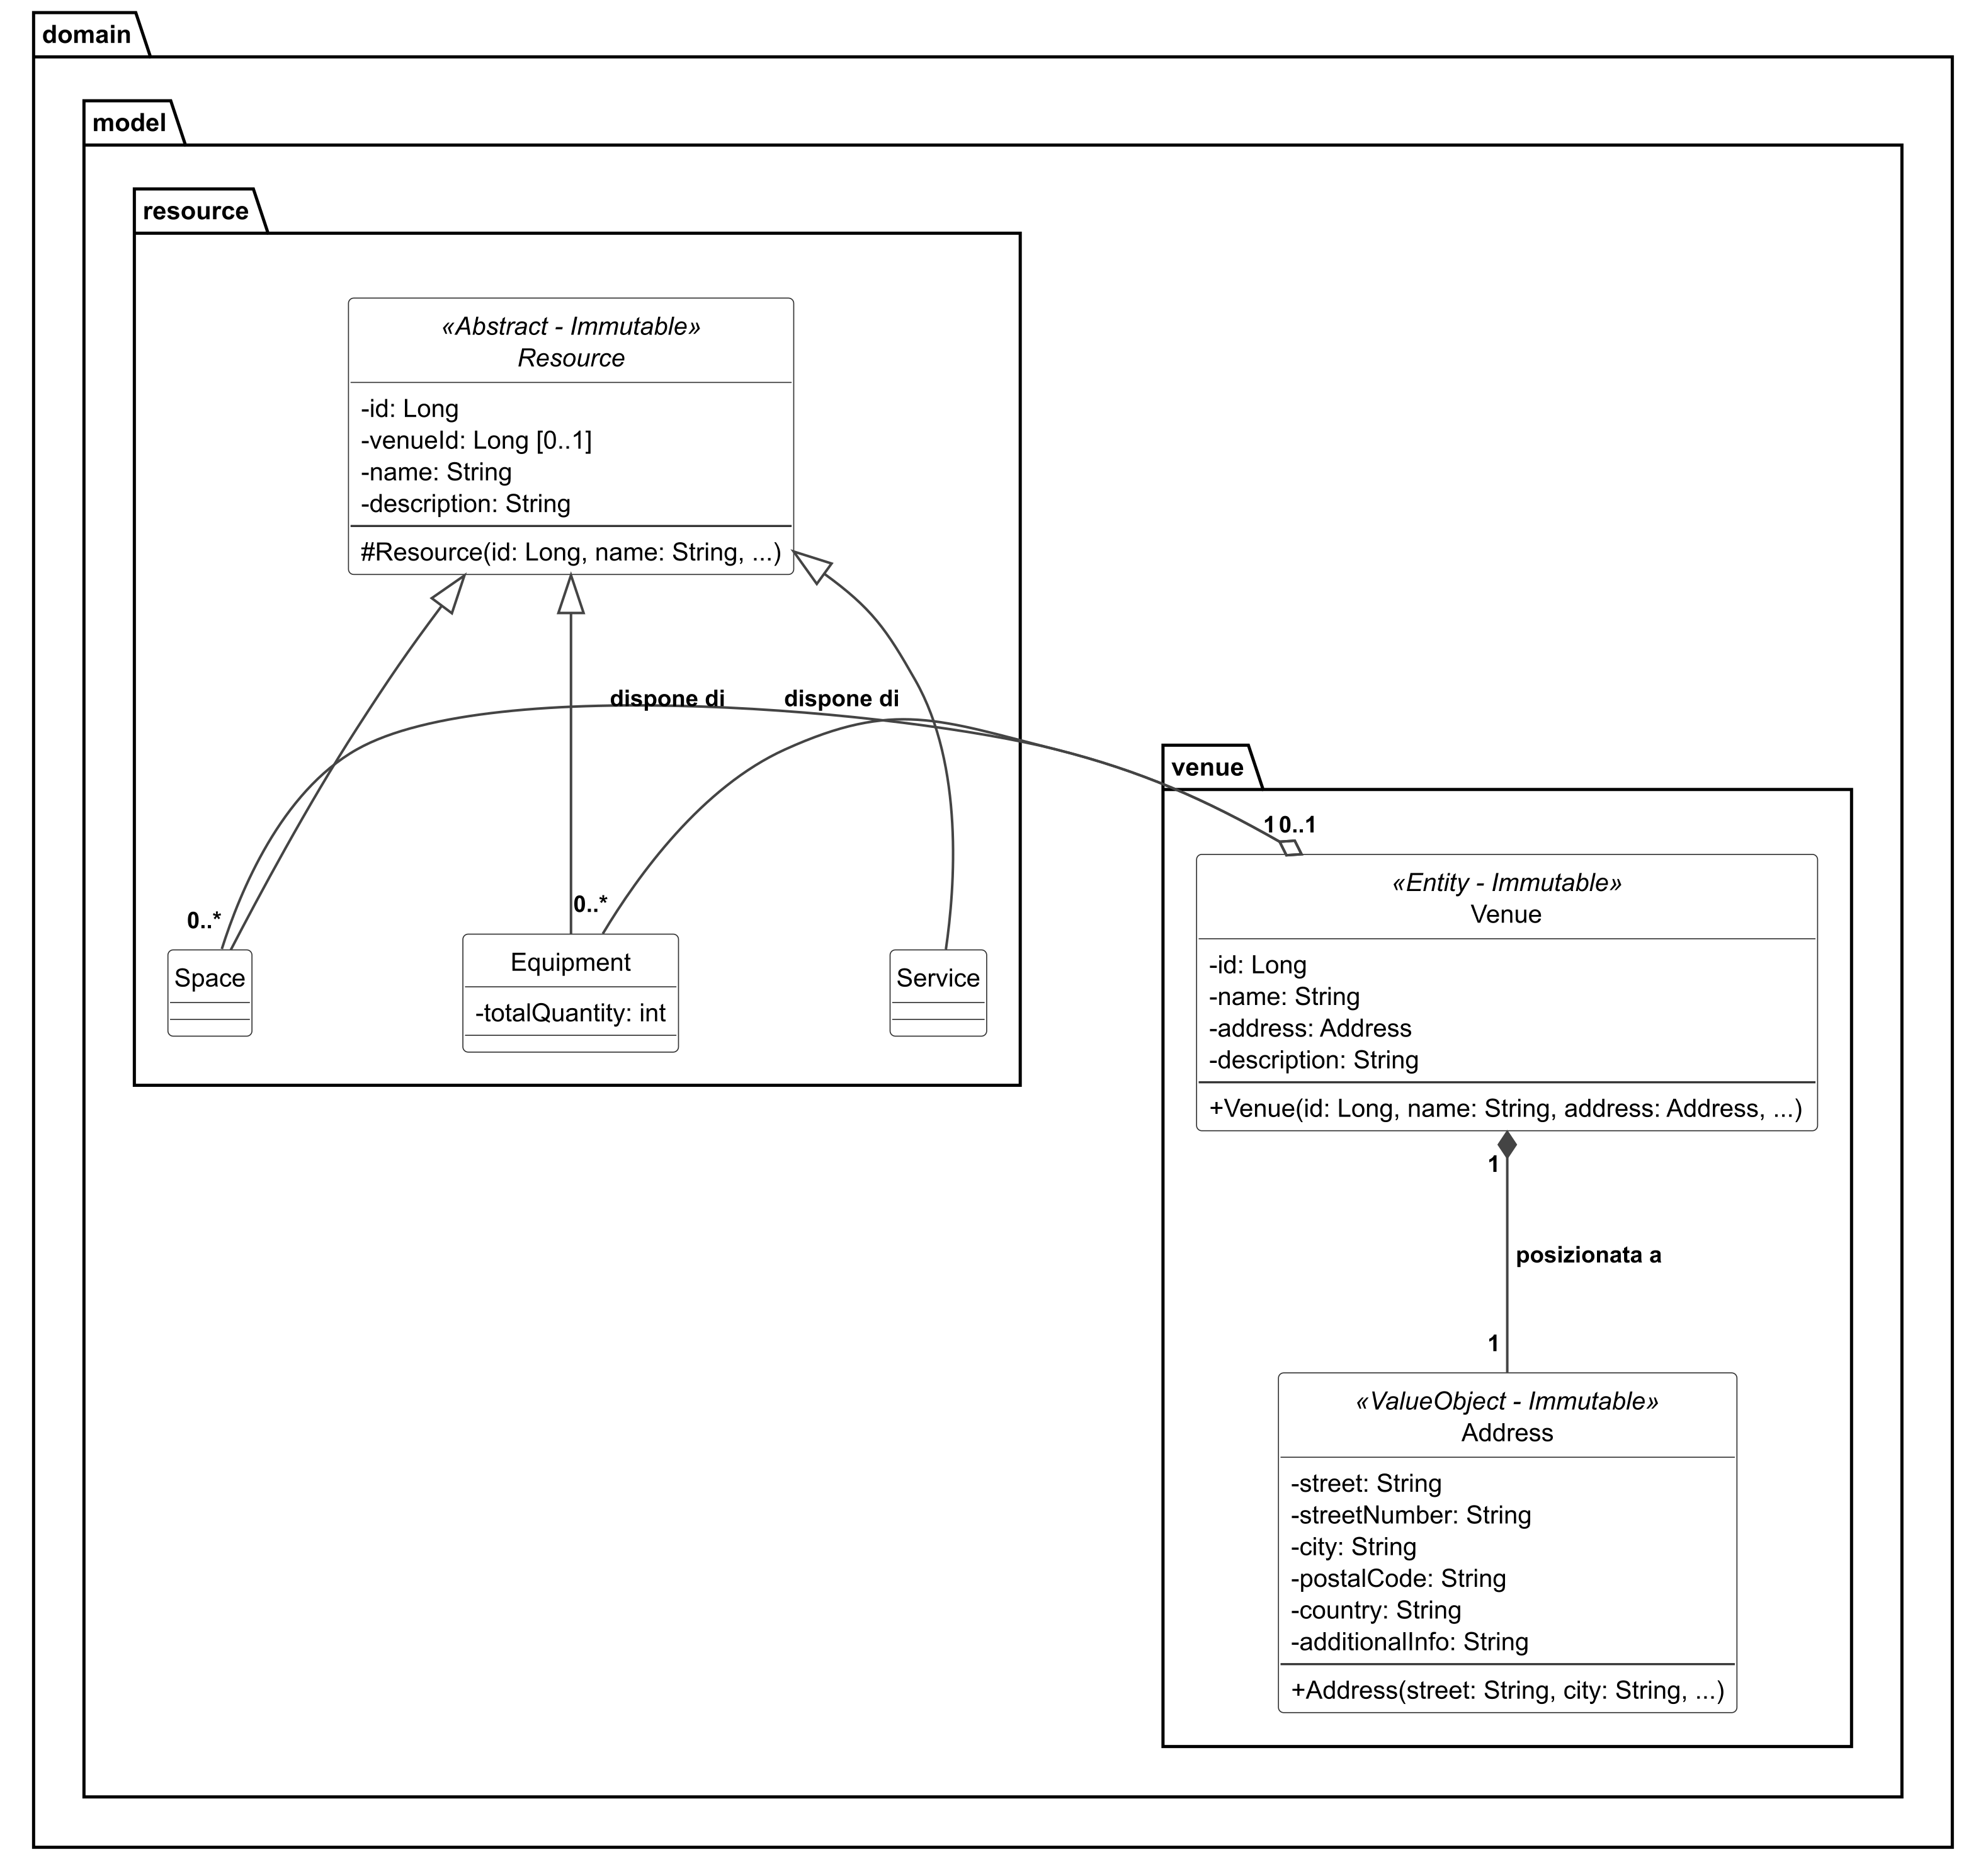
\includegraphics[width=\textwidth,height=0.55\textheight,keepaspectratio]{dominio/domain-venues.png}
  \caption{Diagramma del dominio: venue e risorse.}
  \label{fig:dominio-risorse}
\end{figure}
\FloatBarrier
\par\medskip

\subsection{Richieste di evento}
\label{sec:dominio-richieste}
Un utente ordinario può inviare una \texttt{EventRequest} per richiedere la creazione di un evento in una venue. L'identificativo di tale utente è salvato nel campo \texttt{requester\_id}. La richiesta contiene i dati dell'evento che si vorrebbe organizzare, quali nome, descrizione, data e ora di inizio e di fine, e \texttt{EventRequestStatus} (che può assumere come valori \texttt{PENDING}, \texttt{ACCEPTED}, \texttt{REJECTED} o \texttt{CANCELLED}). Il campo \texttt{handler\_id} indica l'amministratore che ha preso in
carico la richiesta dell'evento. L'accettazione di una richiesta non crea automaticamente un evento, ma indica solamente che la richiesta è stata accettata ed è in fase di valutazione interna. È previsto un campo \texttt{quote} che rappresenta la cifra proposta nel preventivo per la realizzazione dell'evento.
Una richiesta evento deve essere collegata necessariamente a una \texttt{venue}. La richiesta evento deve includere la data e ora di inizio e di fine dell'evento (rispettivamente \texttt{begin\_datetime} e \texttt{end\_datetime}).
\bozza{Descrivere richiedente, venue e handler facoltativo; chiarire che
l'accettazione di una richiesta non crea automaticamente un evento.}
\par\medskip

\subsection{Eventi, prenotazioni, invitati e recensioni}
\label{sec:dominio-eventi}
\bozza{Descrivere creator e organiser, visibilità dell'evento, Booking e Ticket;
distinguere gli invitati privati dagli utenti registrati e spiegare Review.
}
\begin{landscape}
\begin{figure}[p]
  \centering
  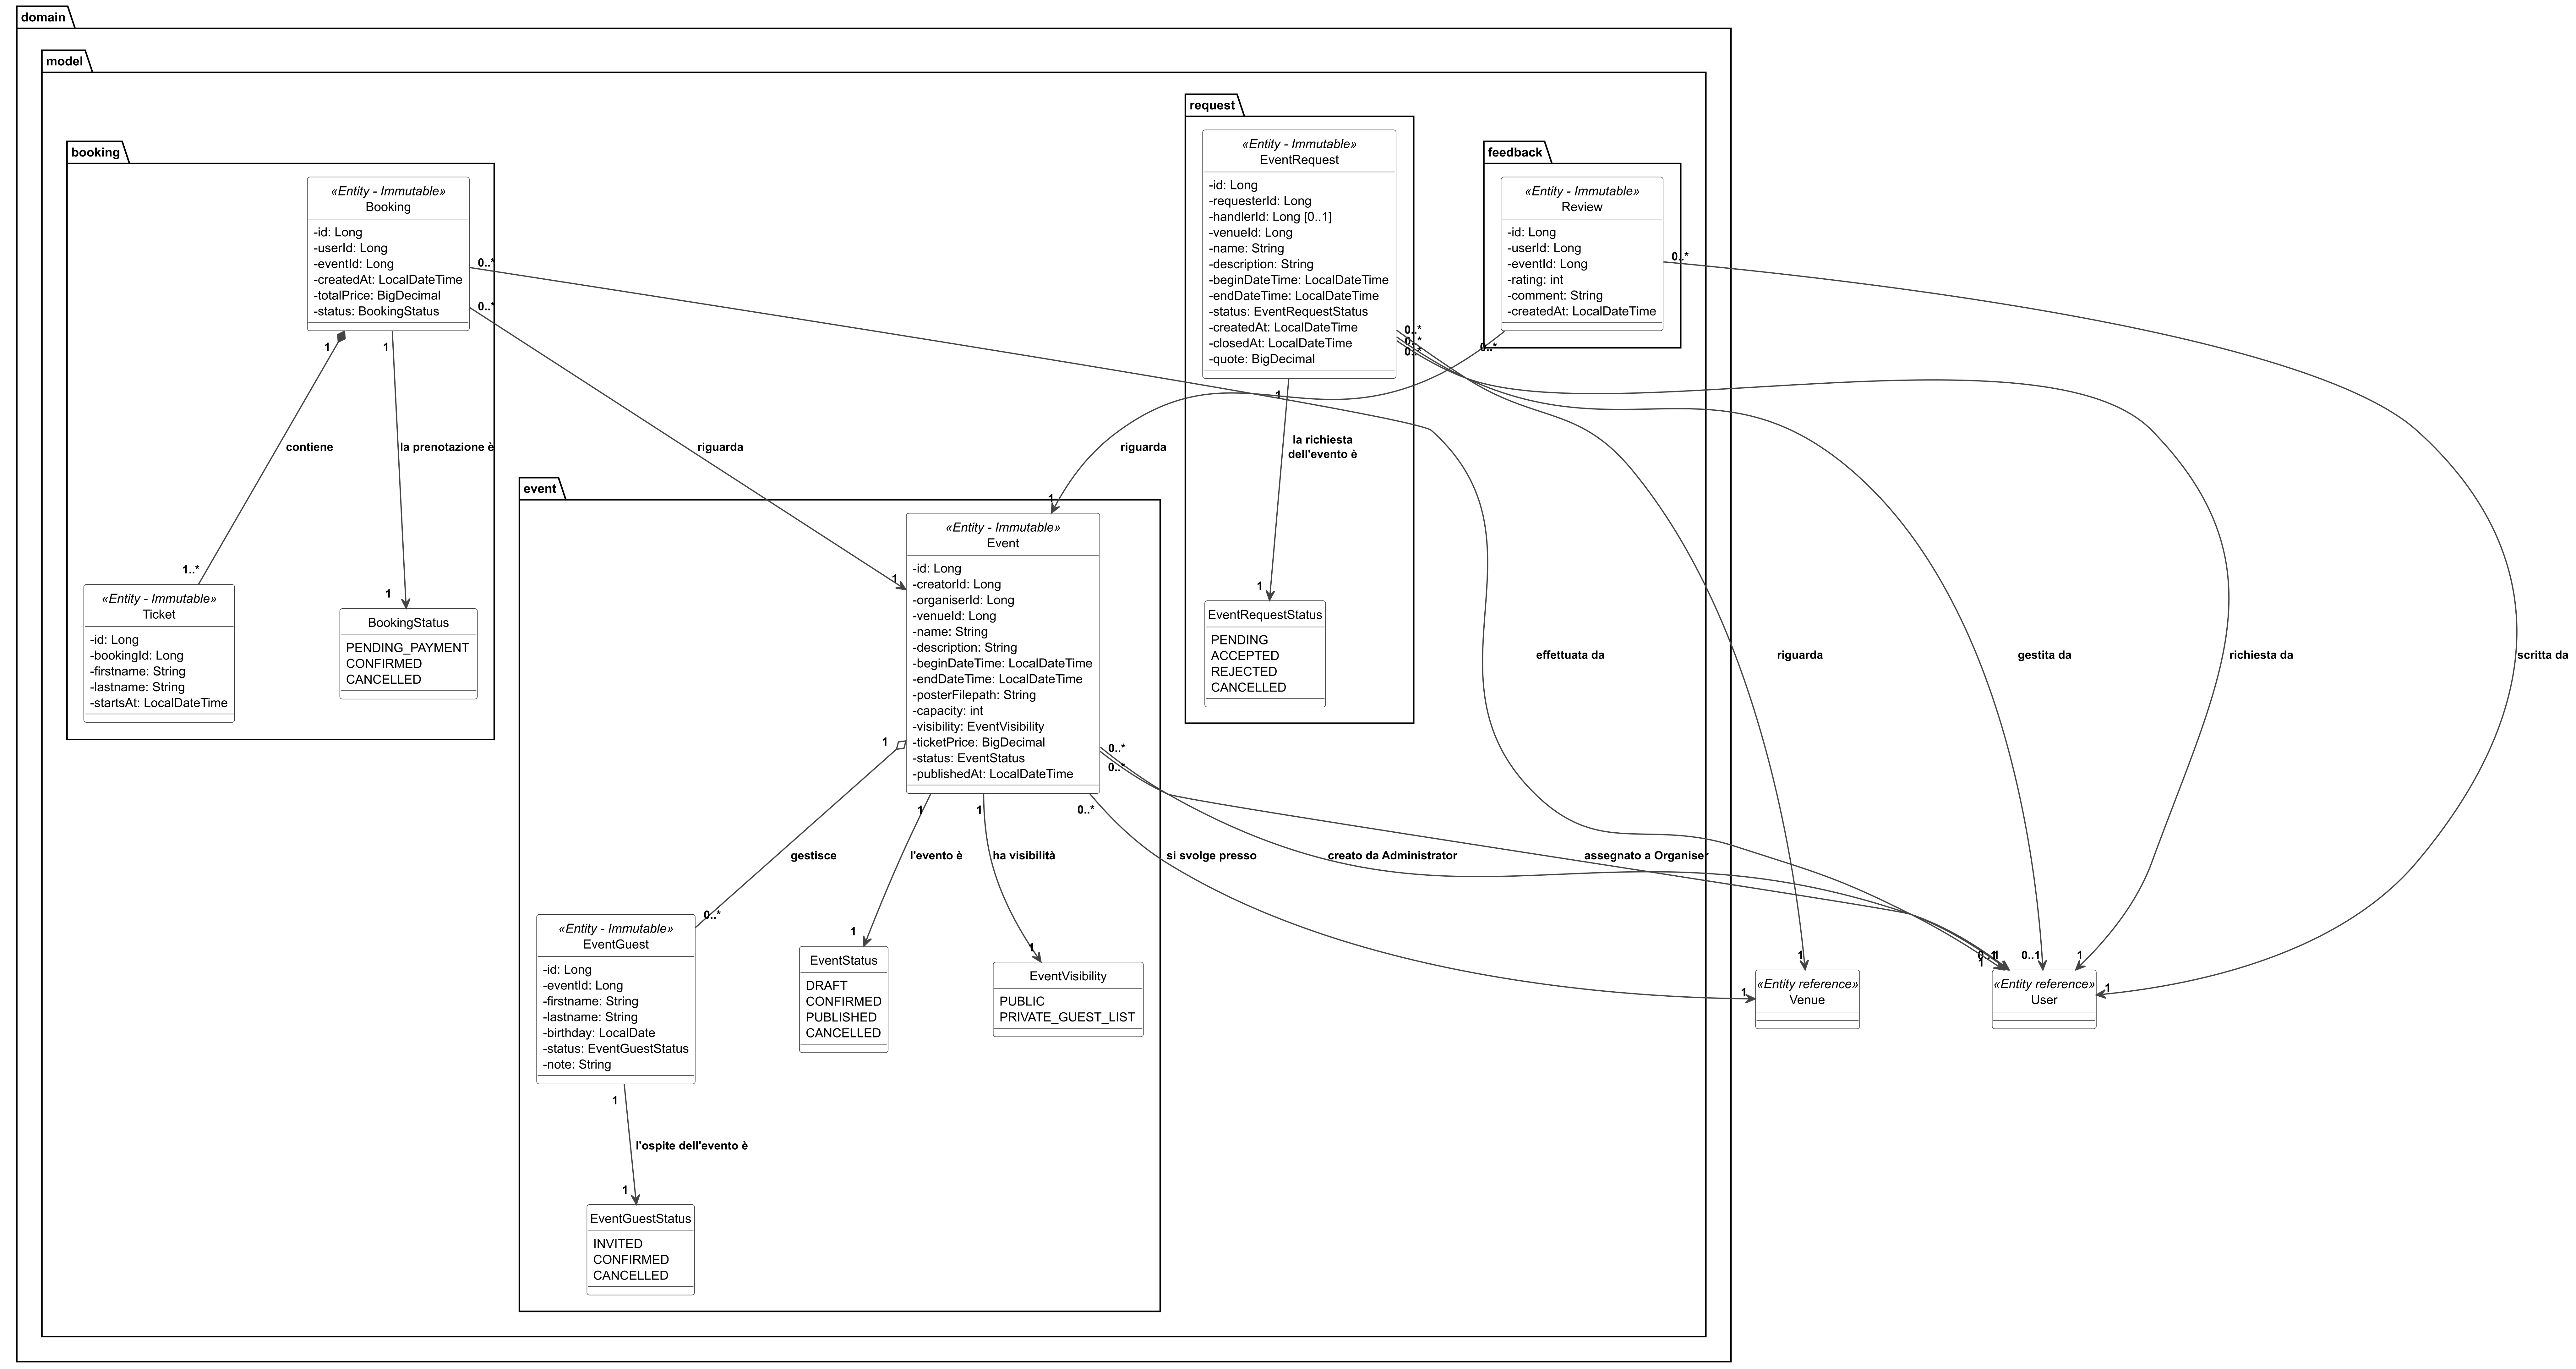
\includegraphics[width=\linewidth,height=0.86\textheight,keepaspectratio]{dominio/domain-events-bookings.png}
  \caption{Diagramma del dominio: richieste, eventi, prenotazioni,
  invitati e recensioni.}
  \label{fig:dominio-eventi}
\end{figure}
\end{landscape}
\par\medskip

\section{Cicli di vita e invarianti}
% Diagrammi originali in docs/diagrams/states/, senza modifiche al contenuto.
\bozza{Introdurre stati, transizioni, guardie ed effetti; richiamare gli ID delle
regole pertinenti senza ricopiare i template dei casi d'uso.}

\subsection{Ciclo di vita dell'evento}
\bozza{Spiegare creazione in DRAFT, conferma, condizioni di pubblicazione e
cancellazione atomica di prenotazioni e inviti. La gestione richiede Administrator
o Organiser assegnato; CANCELLED non consente riattivazione.}
\begin{figure}[!htbp]
  \centering
  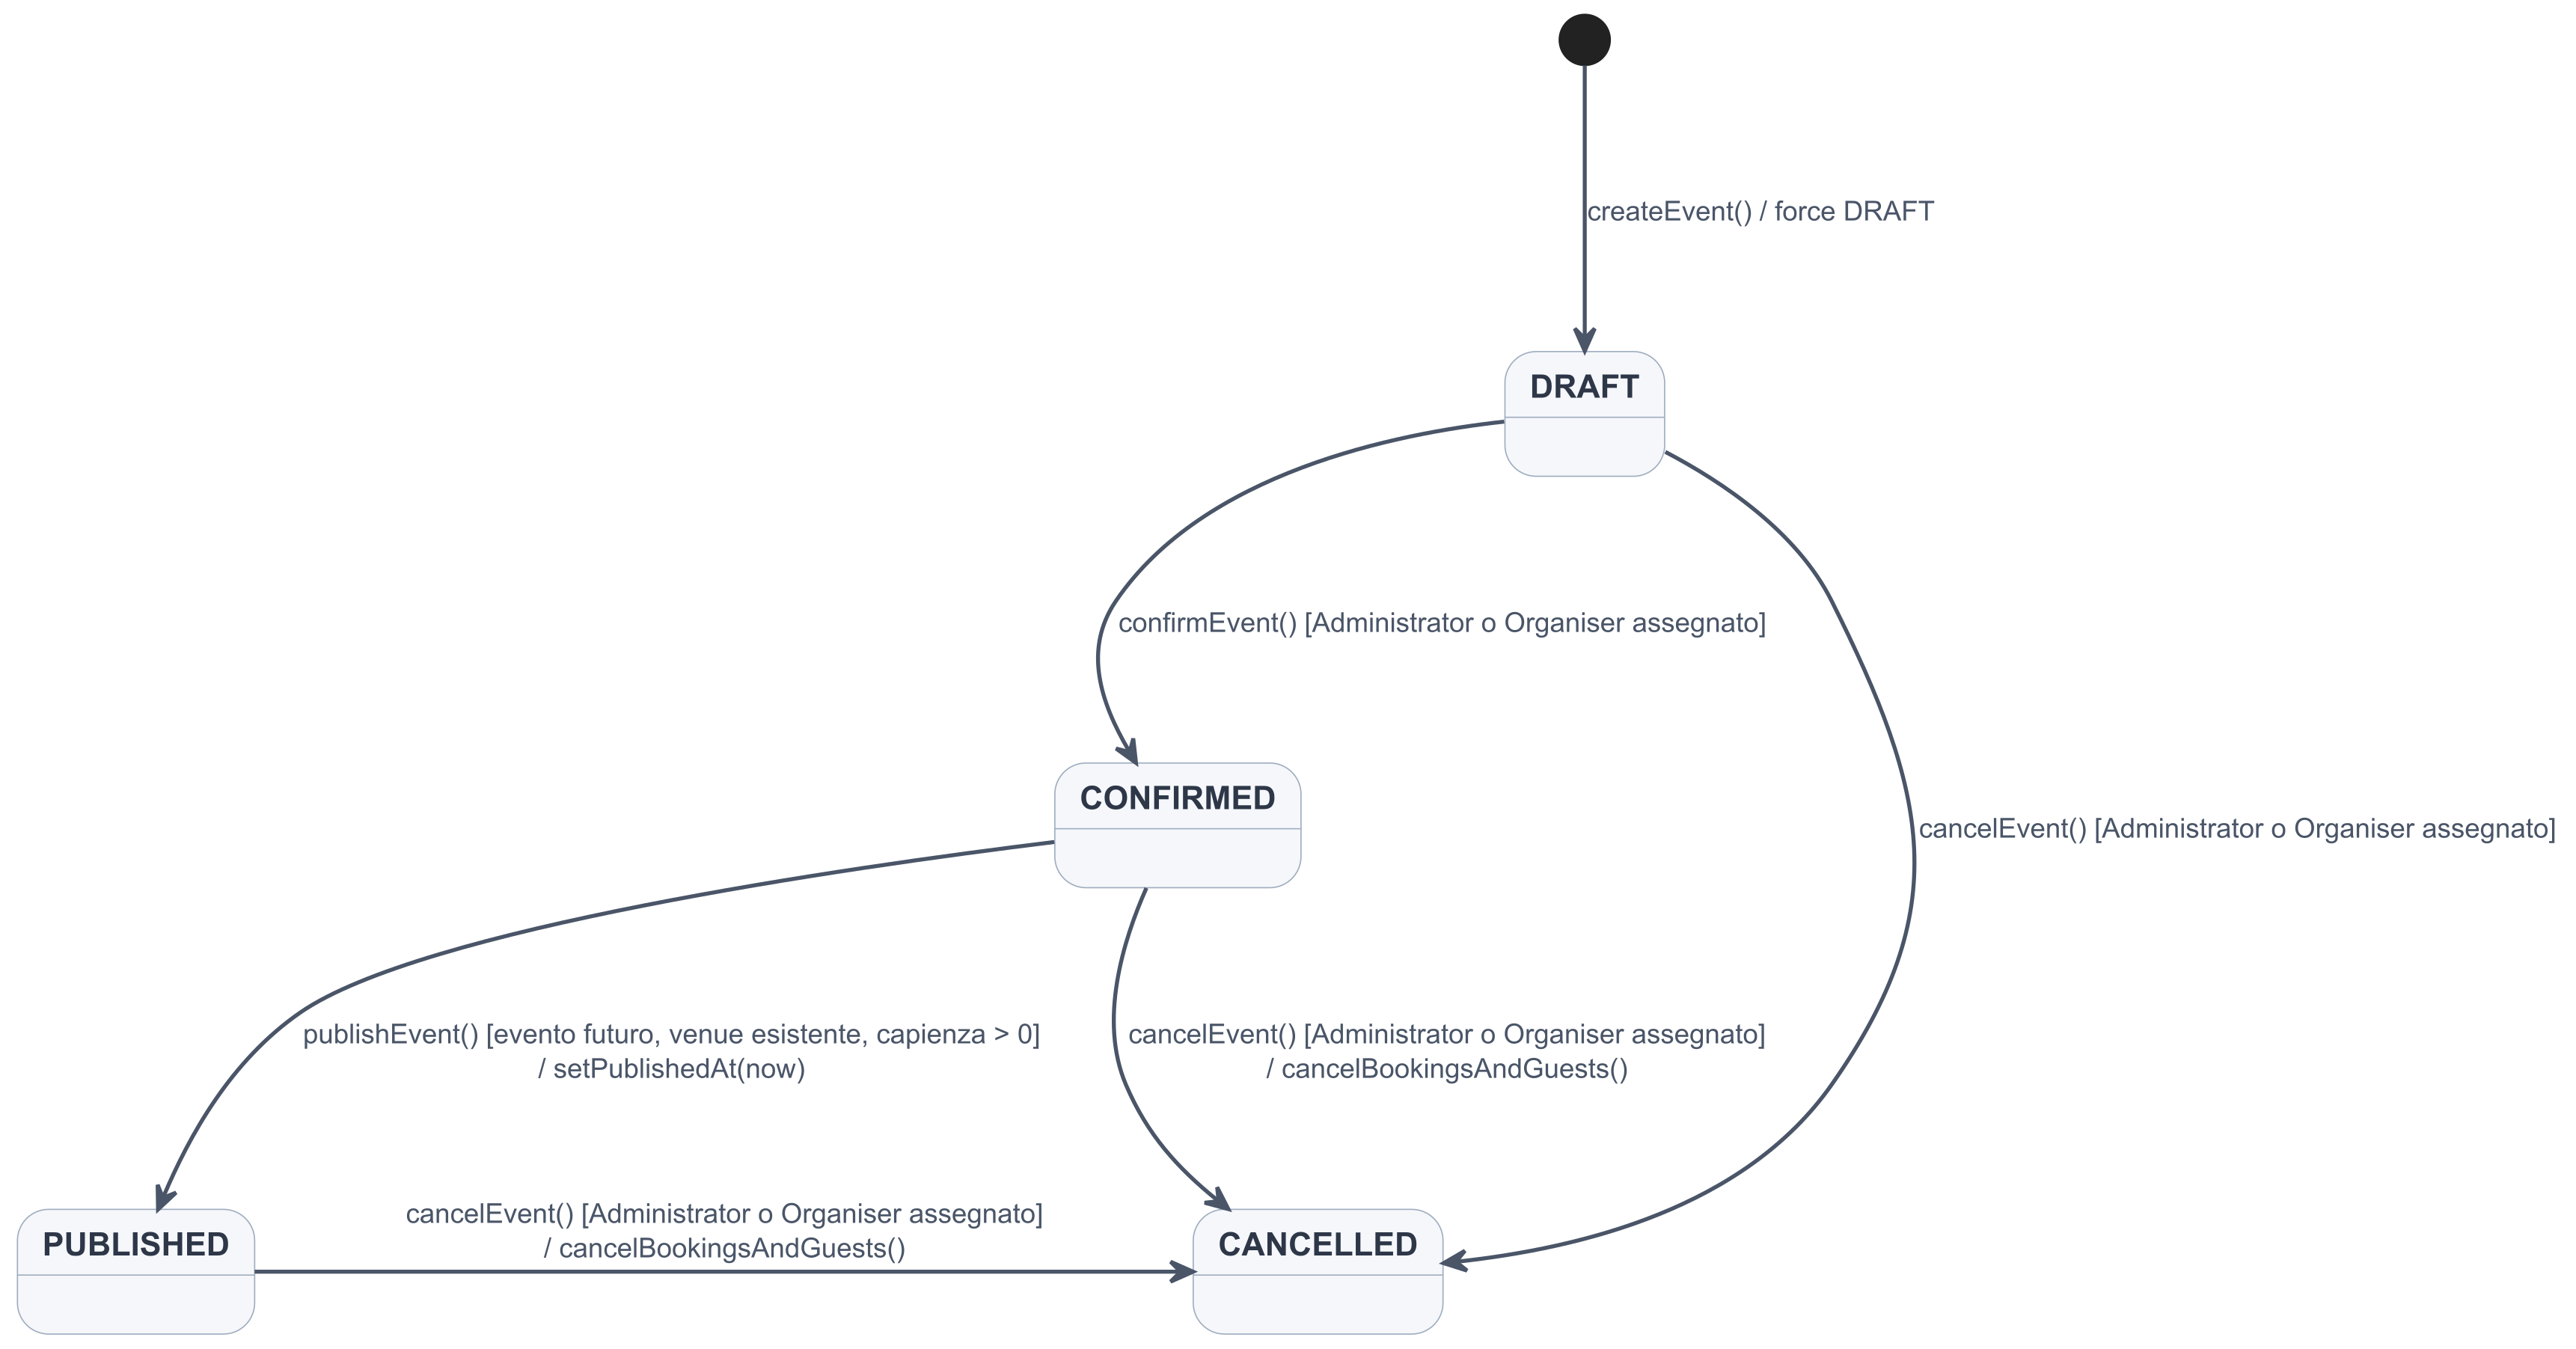
\includegraphics[width=\textwidth,height=0.64\textheight,keepaspectratio]{stati/state-event.png}
  \caption{Diagramma del ciclo di vita dell'evento.}
  \label{fig:stati-evento}
\end{figure}
\FloatBarrier
\par\medskip

\subsection{Ciclo di vita della richiesta}
\bozza{Descrivere assegnazione dell'handler senza cambio di stato e tre possibili
chiusure da PENDING; tutte valorizzano closedAt. ACCEPTED non equivale a un evento creato.}
\begin{figure}[!htbp]
  \centering
  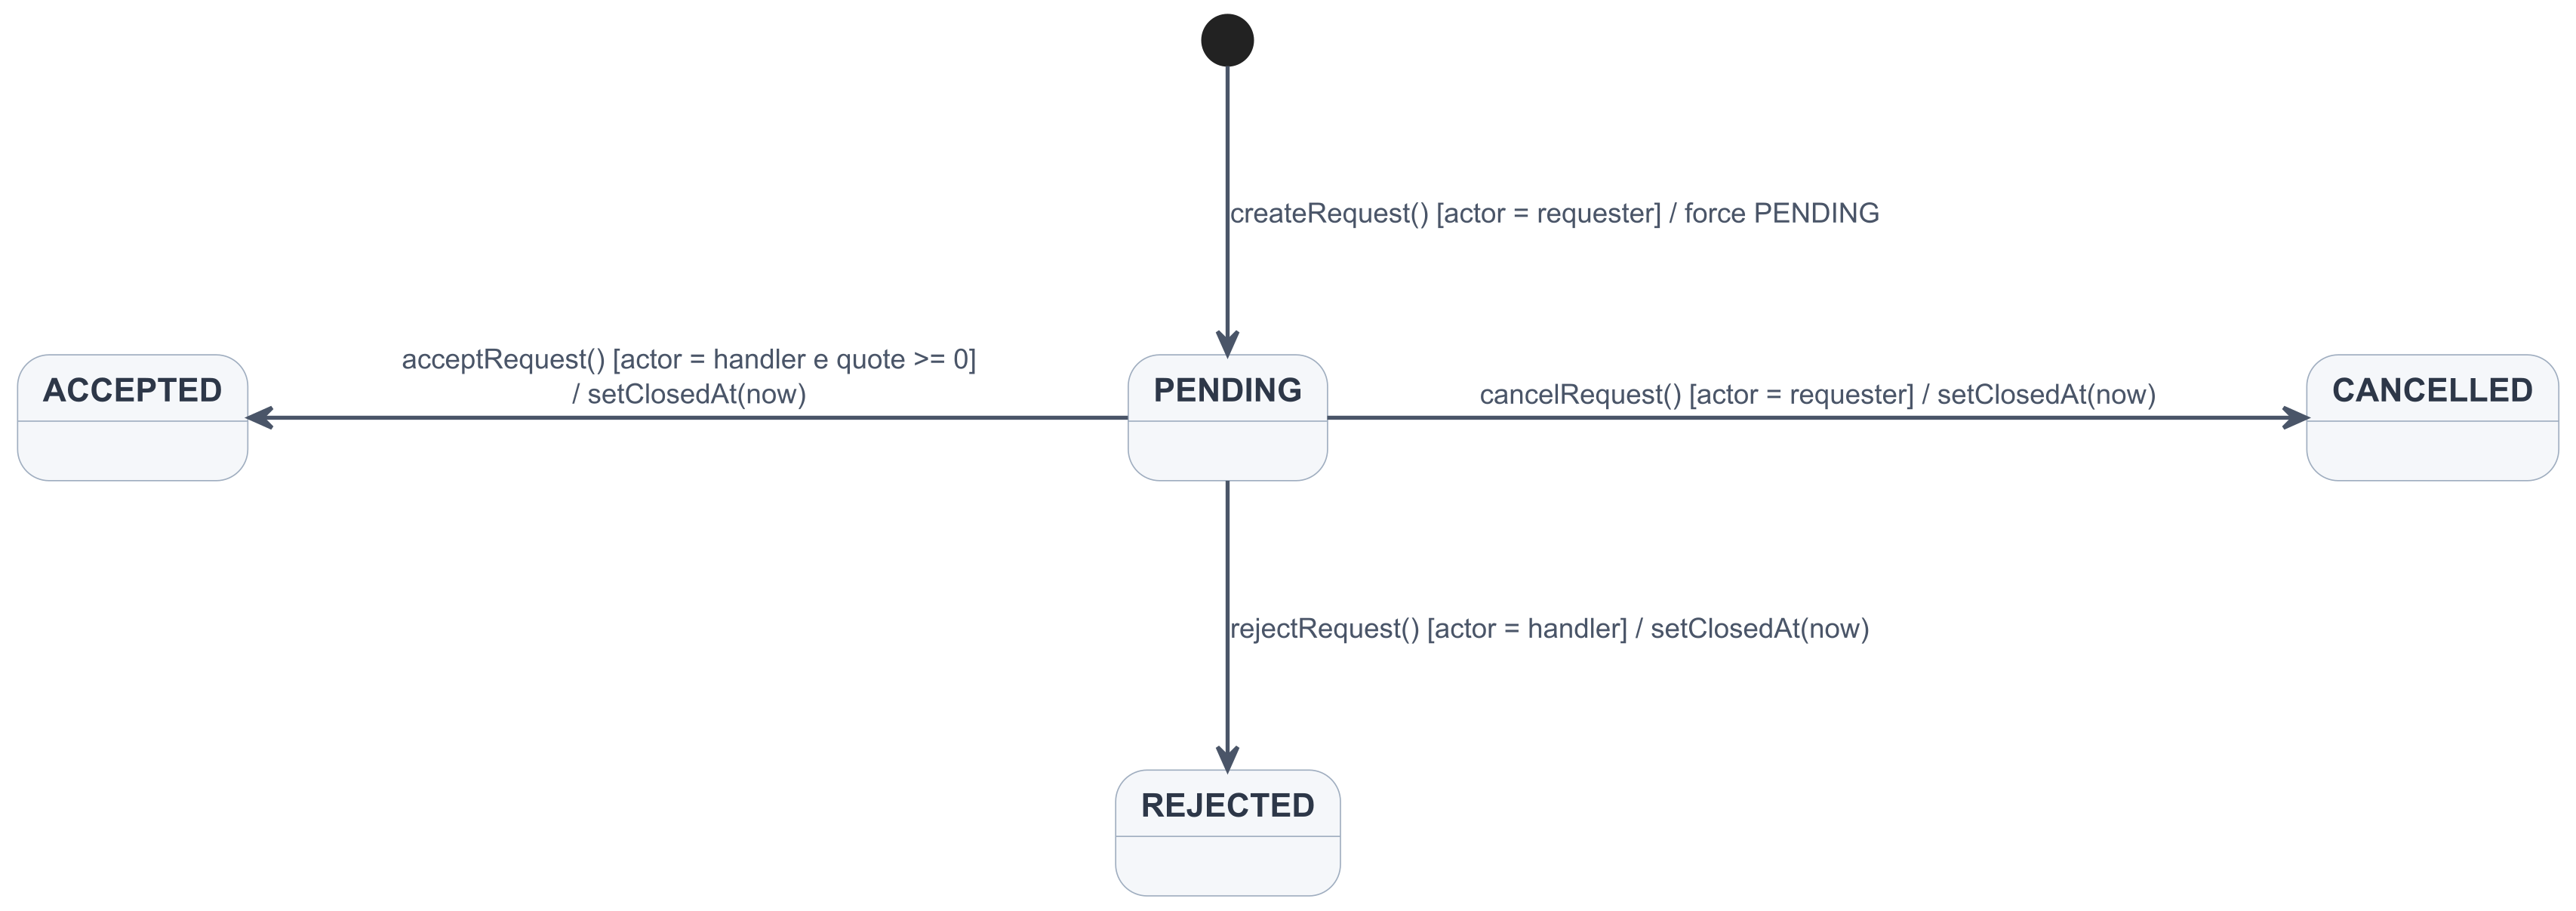
\includegraphics[width=\textwidth,height=0.64\textheight,keepaspectratio]{stati/state-request.png}
  \caption{Diagramma del ciclo di vita della richiesta; le chiusure assegnano closedAt.}
  \label{fig:stati-richiesta}
\end{figure}
\FloatBarrier
\par\medskip

\subsection{Ciclo di vita della prenotazione}
\bozza{Spiegare PENDING\_PAYMENT, conferma e cancellazione; distinguere lo stato
applicativo dall'integrazione con pagamenti reali. Conferma, cancellazione ed
eliminazione richiedono il proprietario o un Administrator.}
\begin{figure}[!htbp]
  \centering
  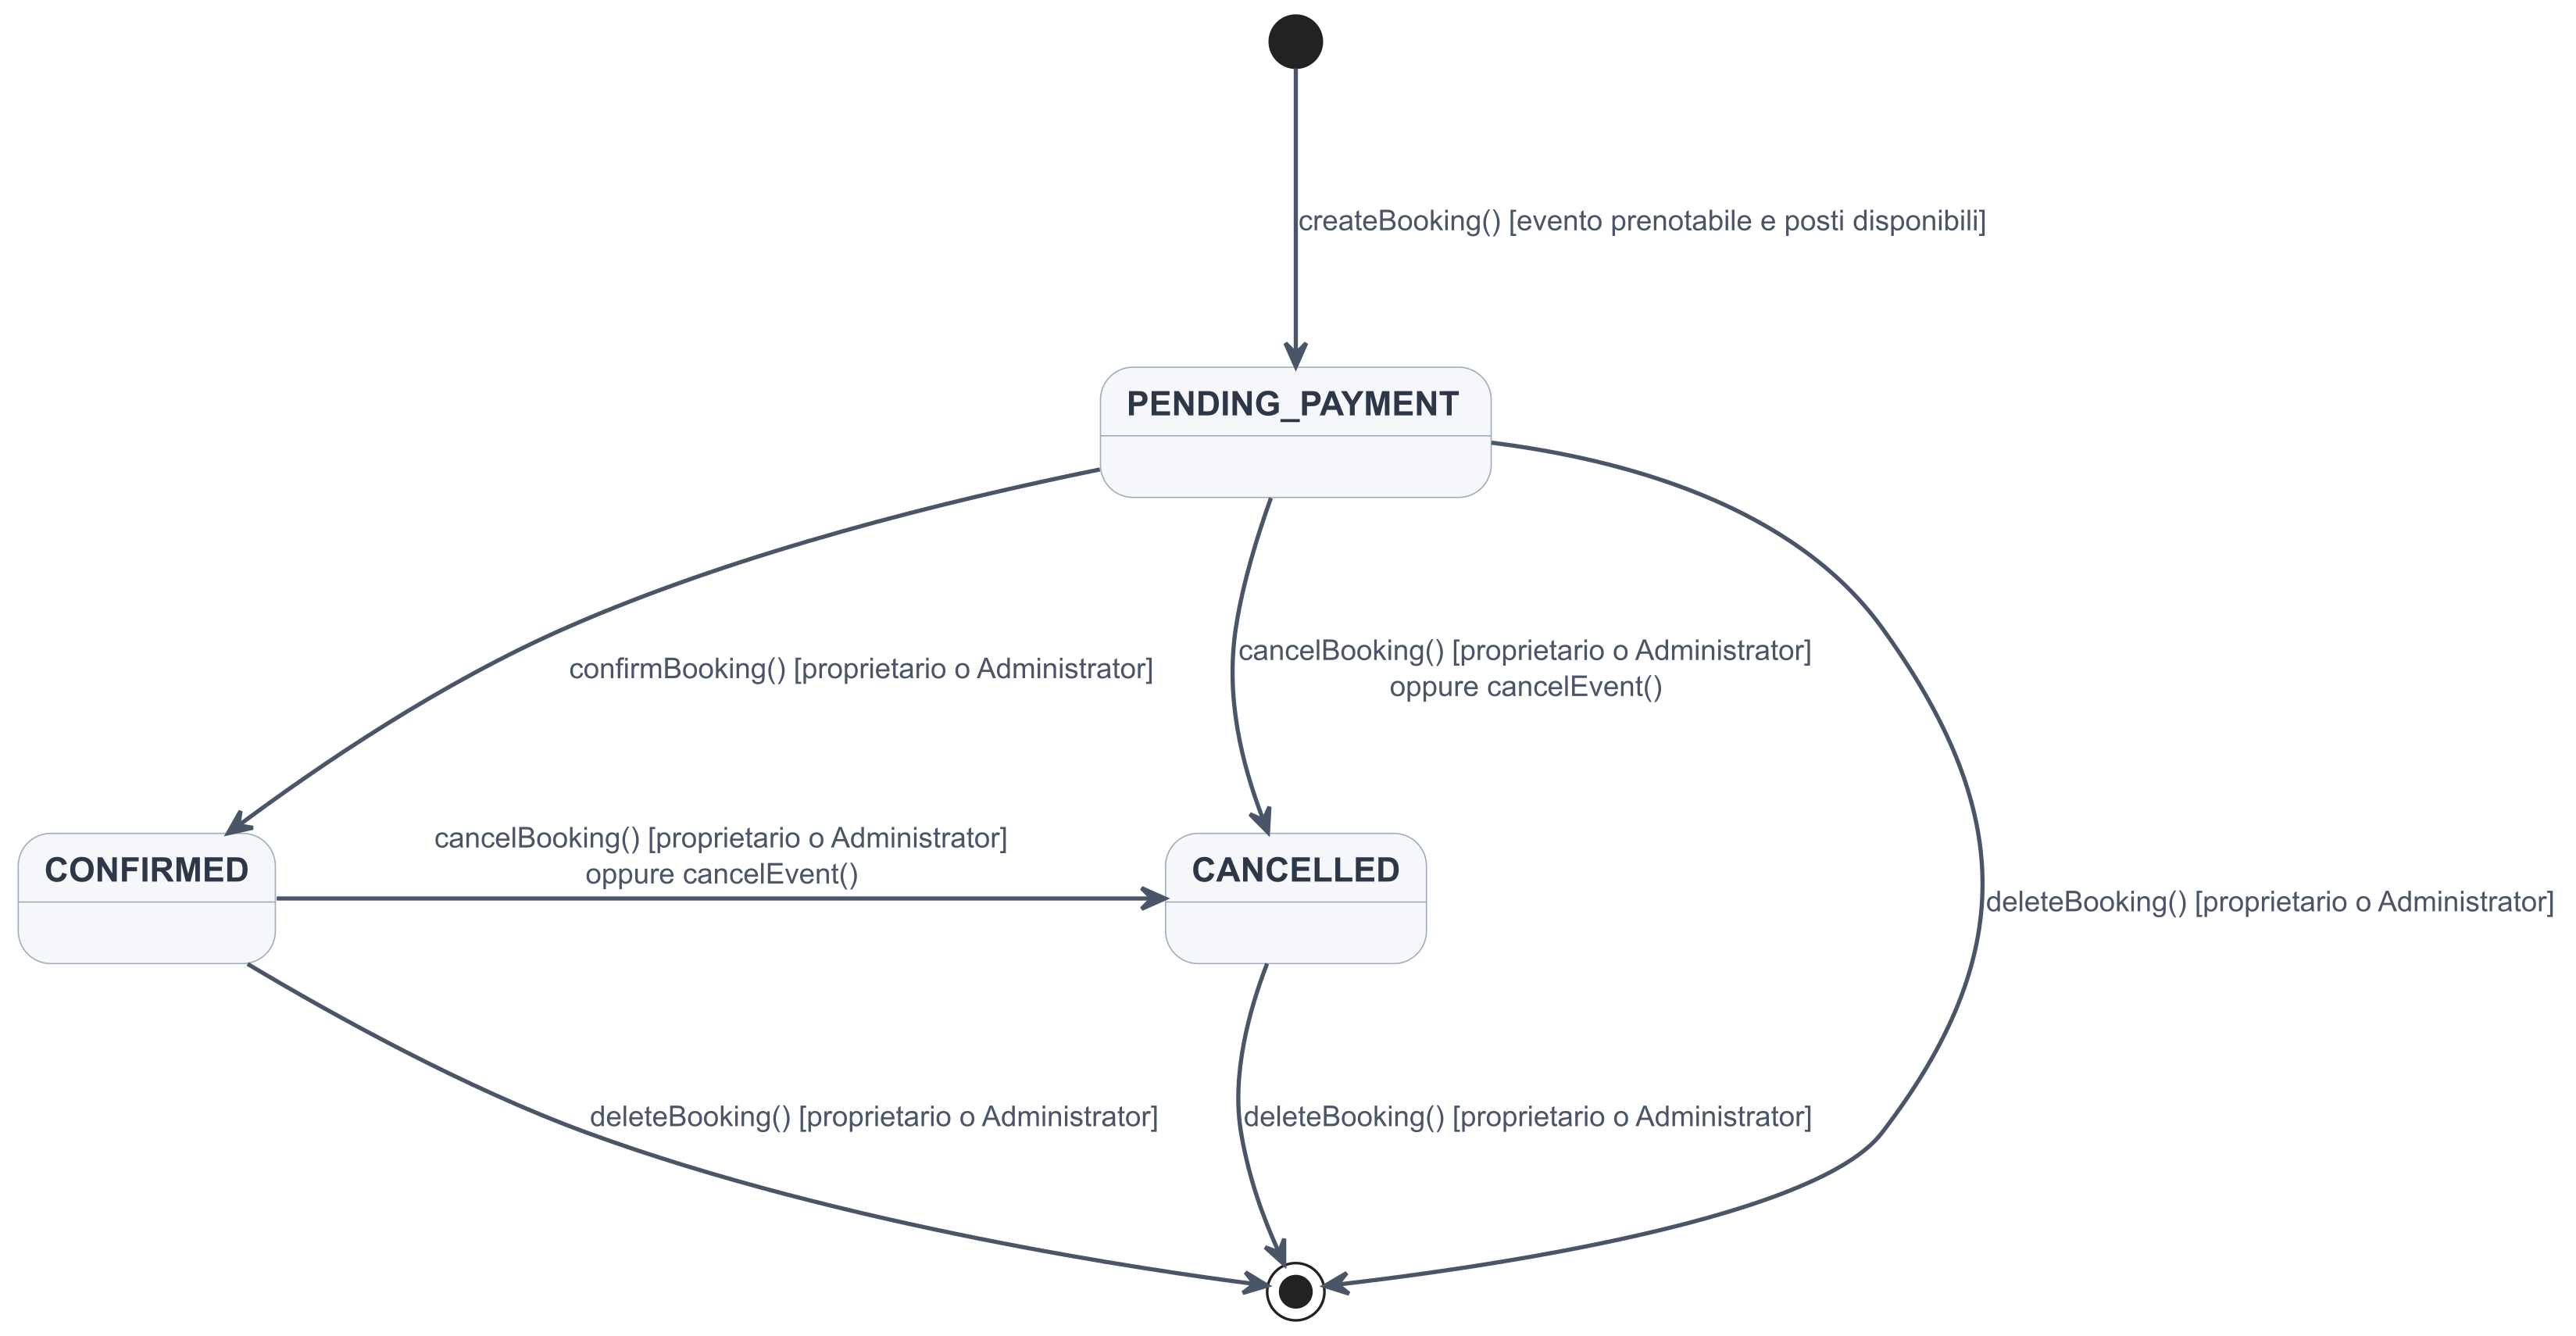
\includegraphics[width=\textwidth,height=0.64\textheight,keepaspectratio]{stati/state-booking.png}
  \caption{Diagramma del ciclo di vita della prenotazione.}
  \label{fig:stati-prenotazione}
\end{figure}
\FloatBarrier
\par\medskip

\subsection{Ciclo di vita dell'invitato}
\bozza{Descrivere INVITED, CONFIRMED e CANCELLED; le operazioni sono registrate
da Administrator o Organiser assegnato. Ricordare l'annullamento degli inviti
attivi quando si cancella l'evento.}
\begin{figure}[!htbp]
  \centering
  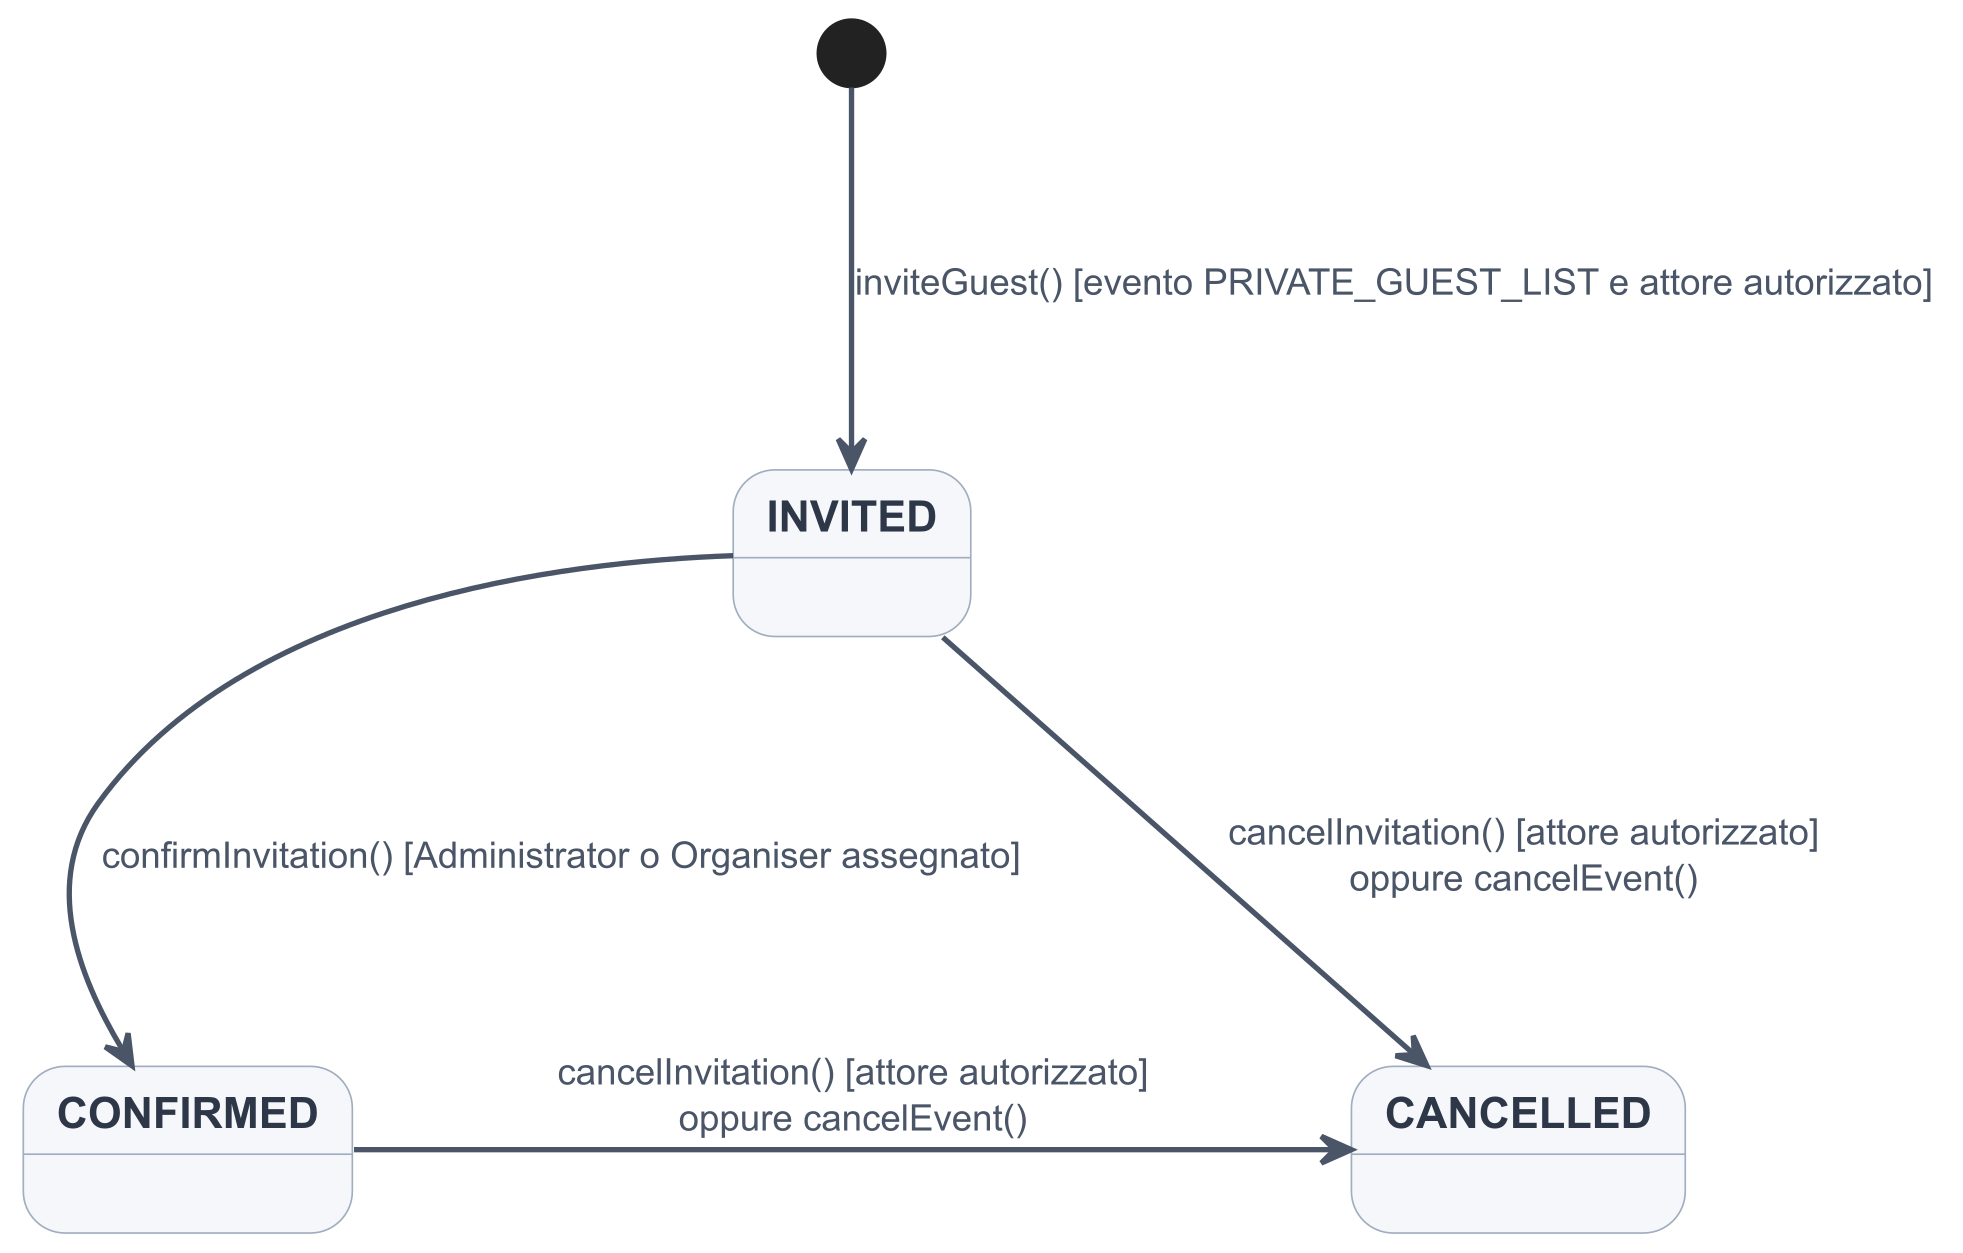
\includegraphics[width=\textwidth,height=0.64\textheight,keepaspectratio]{stati/state-guest.png}
  \caption{Diagramma del ciclo di vita dell'invitato.}
  \label{fig:stati-invitato}
\end{figure}
\FloatBarrier
\par\medskip

\subsection{Ciclo di vita dell'account}
\bozza{Spiegare ACTIVE, ban e riattivazione; il ban impedisce nuove prenotazioni
senza annullare quelle esistenti. Distinguere lo stato BANNED dall'eliminazione
fisica dell'account.}
\begin{figure}[!htbp]
  \centering
  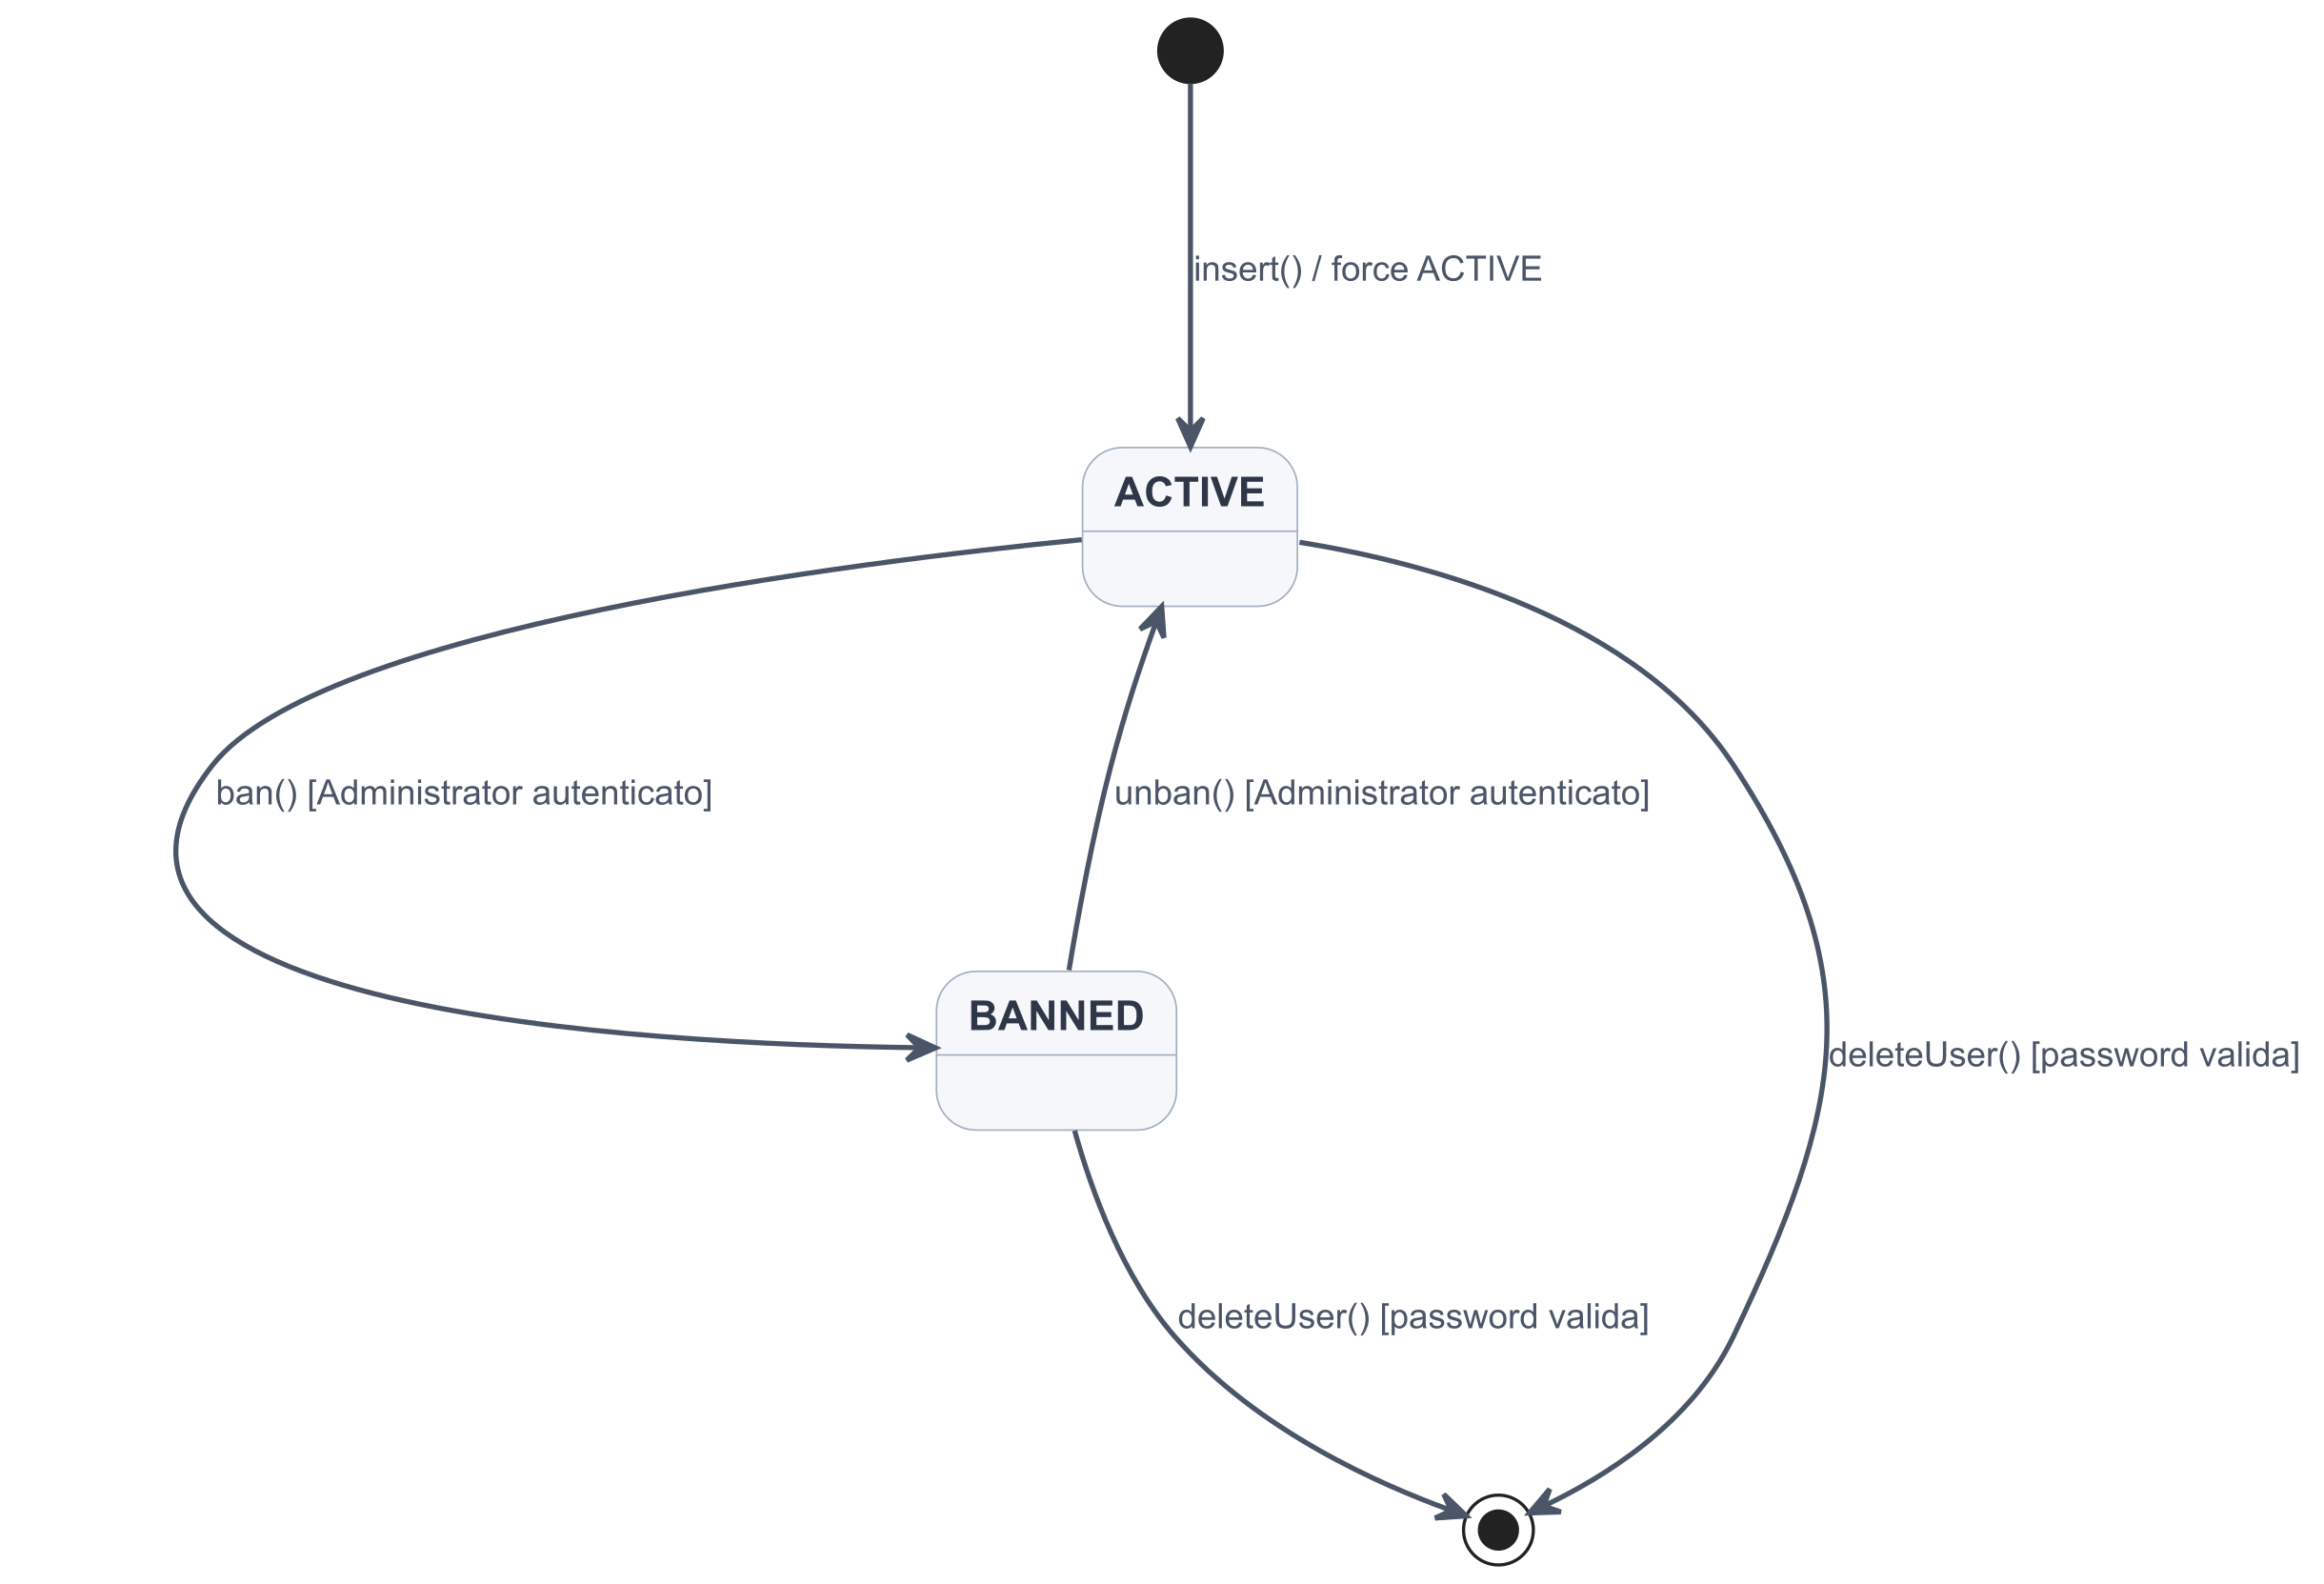
\includegraphics[width=\textwidth,height=0.64\textheight,keepaspectratio]{stati/state-account.png}
  \caption{Diagramma del ciclo di vita dell'account; il nodo finale indica
  l'eliminazione del record.}
  \label{fig:stati-account}
\end{figure}
\FloatBarrier
\par\medskip
